\chapter{Resultados Visuales del Procesamiento}

Más allá de las métricas de rendimiento analizadas en el capítulo anterior, el resultado escencial del proyecto son las imágenes resultantes del pipeline de procesamiento para verificar que las cuatro implementaciones producen una salida visualmente idéntica y para comprender el efecto concreto que cada configuración de filtrado ejerce sobre la imagen original. Las figuras que se presentan a continuación corresponden a la salida de la versión secuencial; las versiones paralelas (OpenMP, MPI e Híbrida) generan resultados pixel-a-pixel equivalentes, dado que el algoritmo de procesamiento es determinístico e independiente del paradigma de concurrencia utilizado.

Para cada una de las tres resoluciones evaluadas ($800 \times 800$, $2000 \times 2000$ y $5000 \times 5000$~píxeles), se contrastan los dos perfiles de filtrado:

\begin{itemize}
    \item \textbf{Perfil liviano} (filtro de $3 \times 3$, 3~niveles de posterizado): produce un efecto visual fuertemente estilizado, con transiciones abruptas entre regiones de color plano. Al disponer de solamente 3~niveles de cuantización por canal, el rango tonal original de la imagen se comprime drásticamente, generando un resultado de aspecto saturado y tipo \textit{pop-art}, donde los degradados suaves de la fotografía original se reemplazan por bloques uniformes de color.
    \item \textbf{Perfil pesado} (filtro de $5 \times 5$, 9~niveles de posterizado): produce un resultado considerablemente más suave y natural. El kernel de mayor tamaño atenúa el ruido de alta frecuencia de forma más agresiva, mientras que los 9~niveles de posterizado preservan un rango tonal significativamente más amplio, permitiendo que los degradados y las transiciones de luminosidad se mantengan con mayor fidelidad respecto de la imagen original.
\end{itemize}


%--------------------------------------------------------------------
\section{Imagen de \texorpdfstring{$800 \times 800$}{800x800} píxeles}

\begin{figure}[H]
    \centering
    \begin{minipage}[t]{0.47\textwidth}
        \centering
        
\includegraphics[width=\textwidth]{../resources/output_800_3_3.jpg}
        \caption{Filtro $3 \times 3$, 3~niveles.}
        \label{fig:out_800_3_3}
    \end{minipage}
    \hfill
    \begin{minipage}[t]{0.47\textwidth}
        \centering
        
\includegraphics[width=\textwidth]{../resources/output_800_5_9.jpg}
        \caption{Filtro $5 \times 5$, 9~niveles.}
        \label{fig:out_800_5_9}
    \end{minipage}
    \caption{Resultados del procesamiento sobre la imagen de $800 \times 800$~píxeles.}
    \label{fig:output_800}
\end{figure}

En la configuración de 3~niveles (Figura~\ref{fig:out_800_3_3}), las zonas de piel y fondo se reducen a parches planos de color con contornos marcados, produciendo un efecto visual similar al de una ilustración vectorial. La configuración de 9~niveles (Figura~\ref{fig:out_800_5_9}), en cambio, conserva los matices tonales del rostro y la textura del fondo, resultando en una imagen que se percibe como una versión estilizada pero fiel de la fotografía original.


%--------------------------------------------------------------------
\section{Imagen de \texorpdfstring{$2000 \times 2000$}{2000x2000} píxeles}

\begin{figure}[H]
    \centering
    \begin{minipage}[t]{0.47\textwidth}
        \centering
        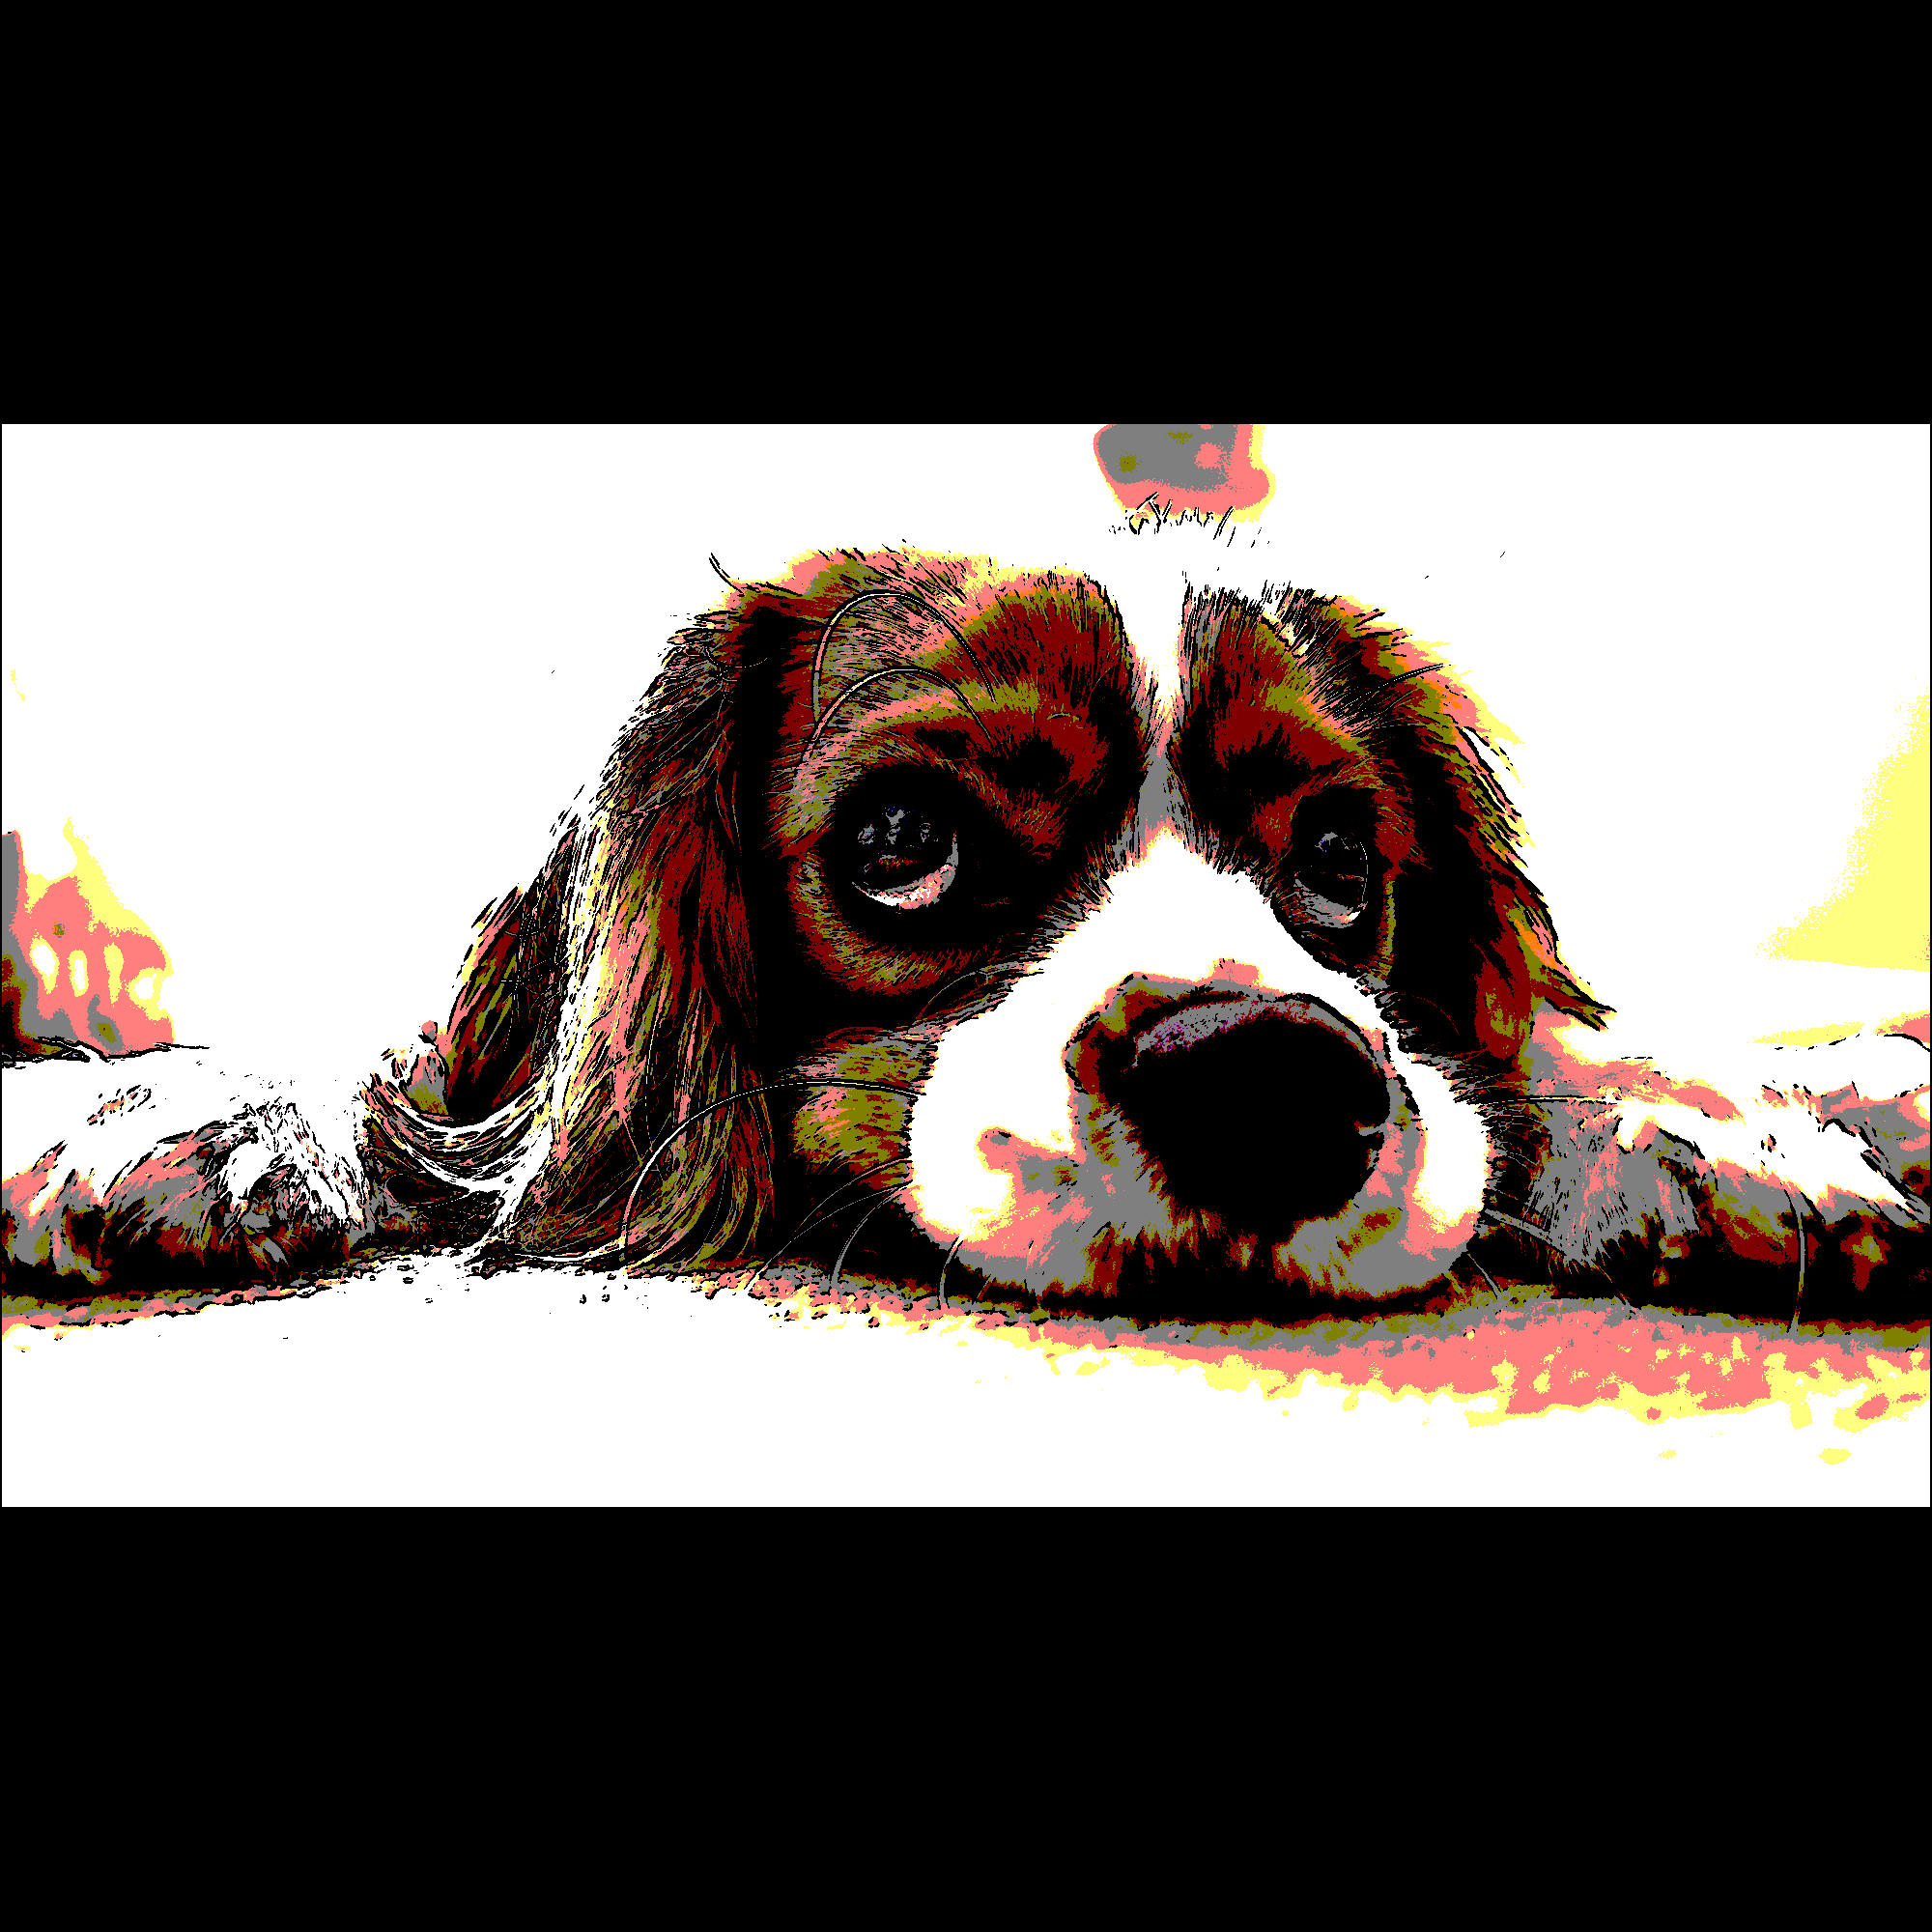
\includegraphics[width=\textwidth]{../resources/output_2000_3_3.jpg}
        \caption{Filtro $3 \times 3$, 3~niveles.}
        \label{fig:out_2000_3_3}
    \end{minipage}
    \hfill
    \begin{minipage}[t]{0.47\textwidth}
        \centering
        
\includegraphics[width=\textwidth]{../resources/output_2000_5_9.jpg}
        \caption{Filtro $5 \times 5$, 9~niveles.}
        \label{fig:out_2000_5_9}
    \end{minipage}
    \caption{Resultados del procesamiento sobre la imagen de $2000 \times 2000$~píxeles.}
    \label{fig:output_2000}
\end{figure}

Al incrementar la resolución, el mayor nivel de detalle espacial acentúa la diferencia perceptual entre ambos perfiles. Con 3~niveles de posterizado (Figura~\ref{fig:out_2000_3_3}), las regiones de tonalidad similar colapsan en áreas extensas de color uniforme, eliminando prácticamente toda textura y generando un aspecto plano y sobresaturado. Con 9~niveles (Figura~\ref{fig:out_2000_5_9}), la mayor granularidad tonal permite que las variaciones sutiles de iluminación y sombra se preserven, manteniendo la profundidad visual y el volumen percibido de los elementos de la imagen.


%--------------------------------------------------------------------
\section{Imagen de \texorpdfstring{$5000 \times 5000$}{5000x5000} píxeles}

\begin{figure}[H]
    \centering
    \begin{minipage}[t]{0.47\textwidth}
        \centering
        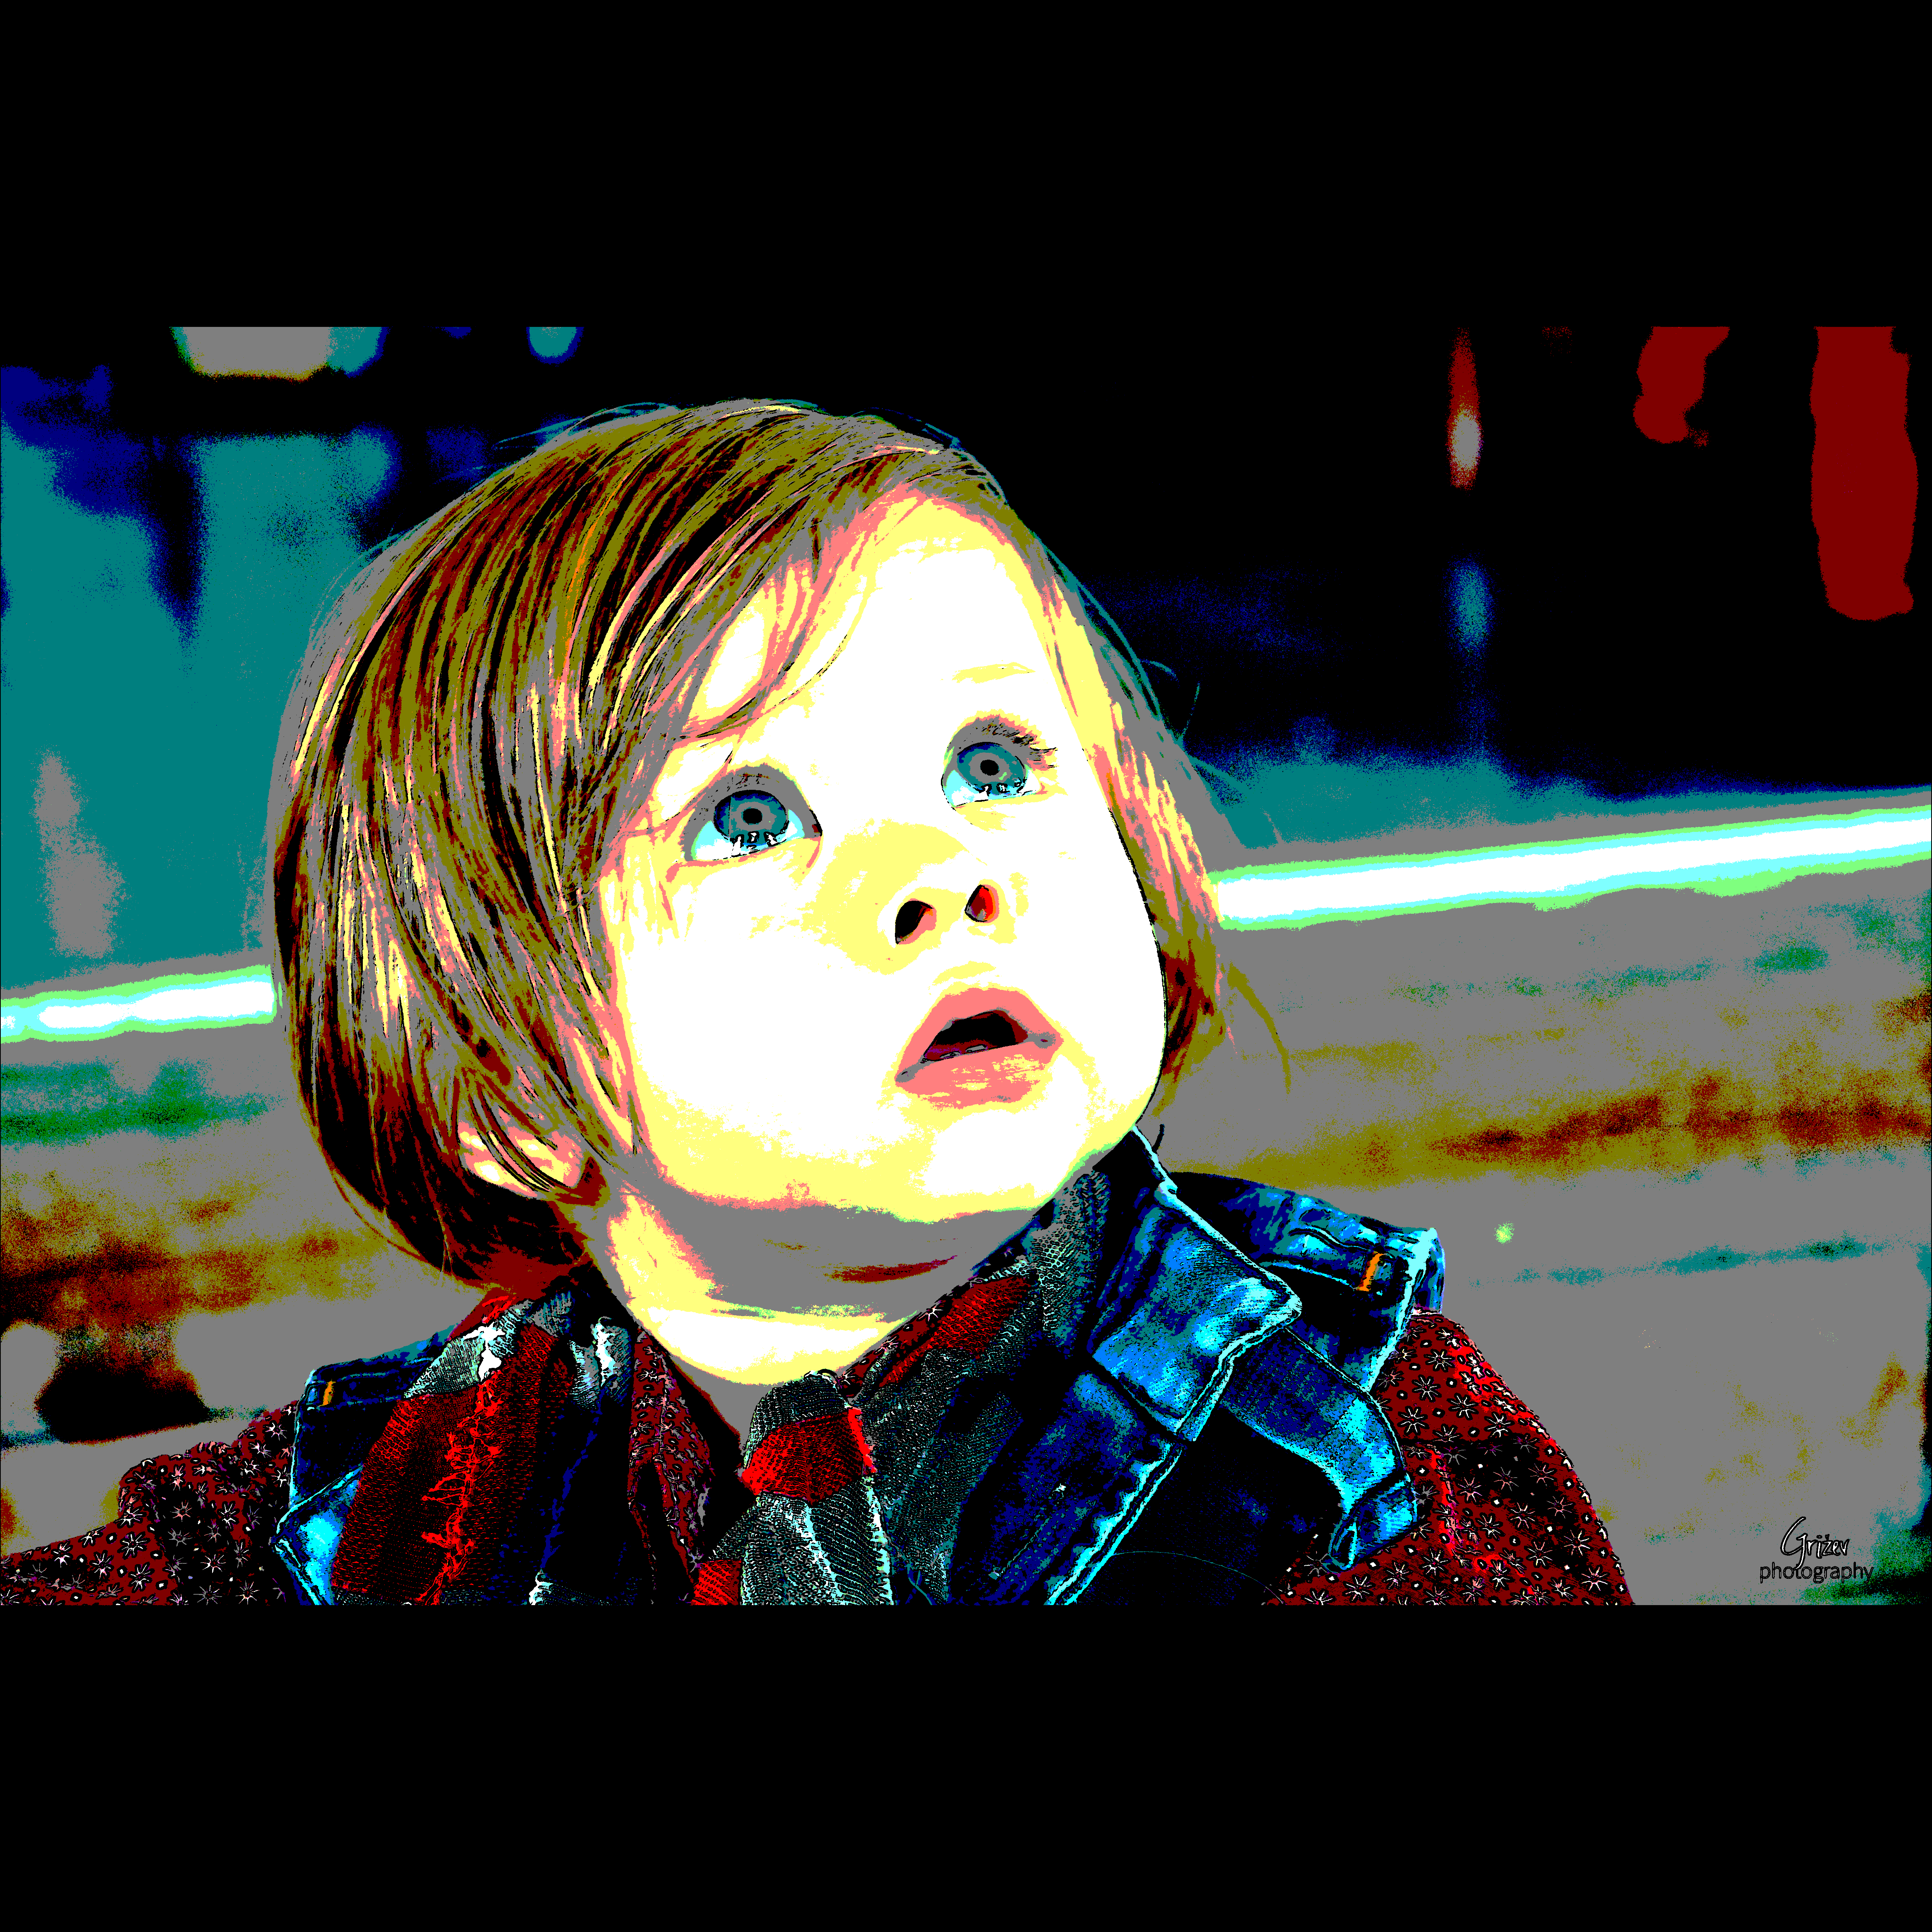
\includegraphics[width=\textwidth]{../resources/output_5000_3_3.jpg}
        \caption{Filtro $3 \times 3$, 3~niveles.}
        \label{fig:out_5000_3_3}
    \end{minipage}
    \hfill
    \begin{minipage}[t]{0.47\textwidth}
        \centering
        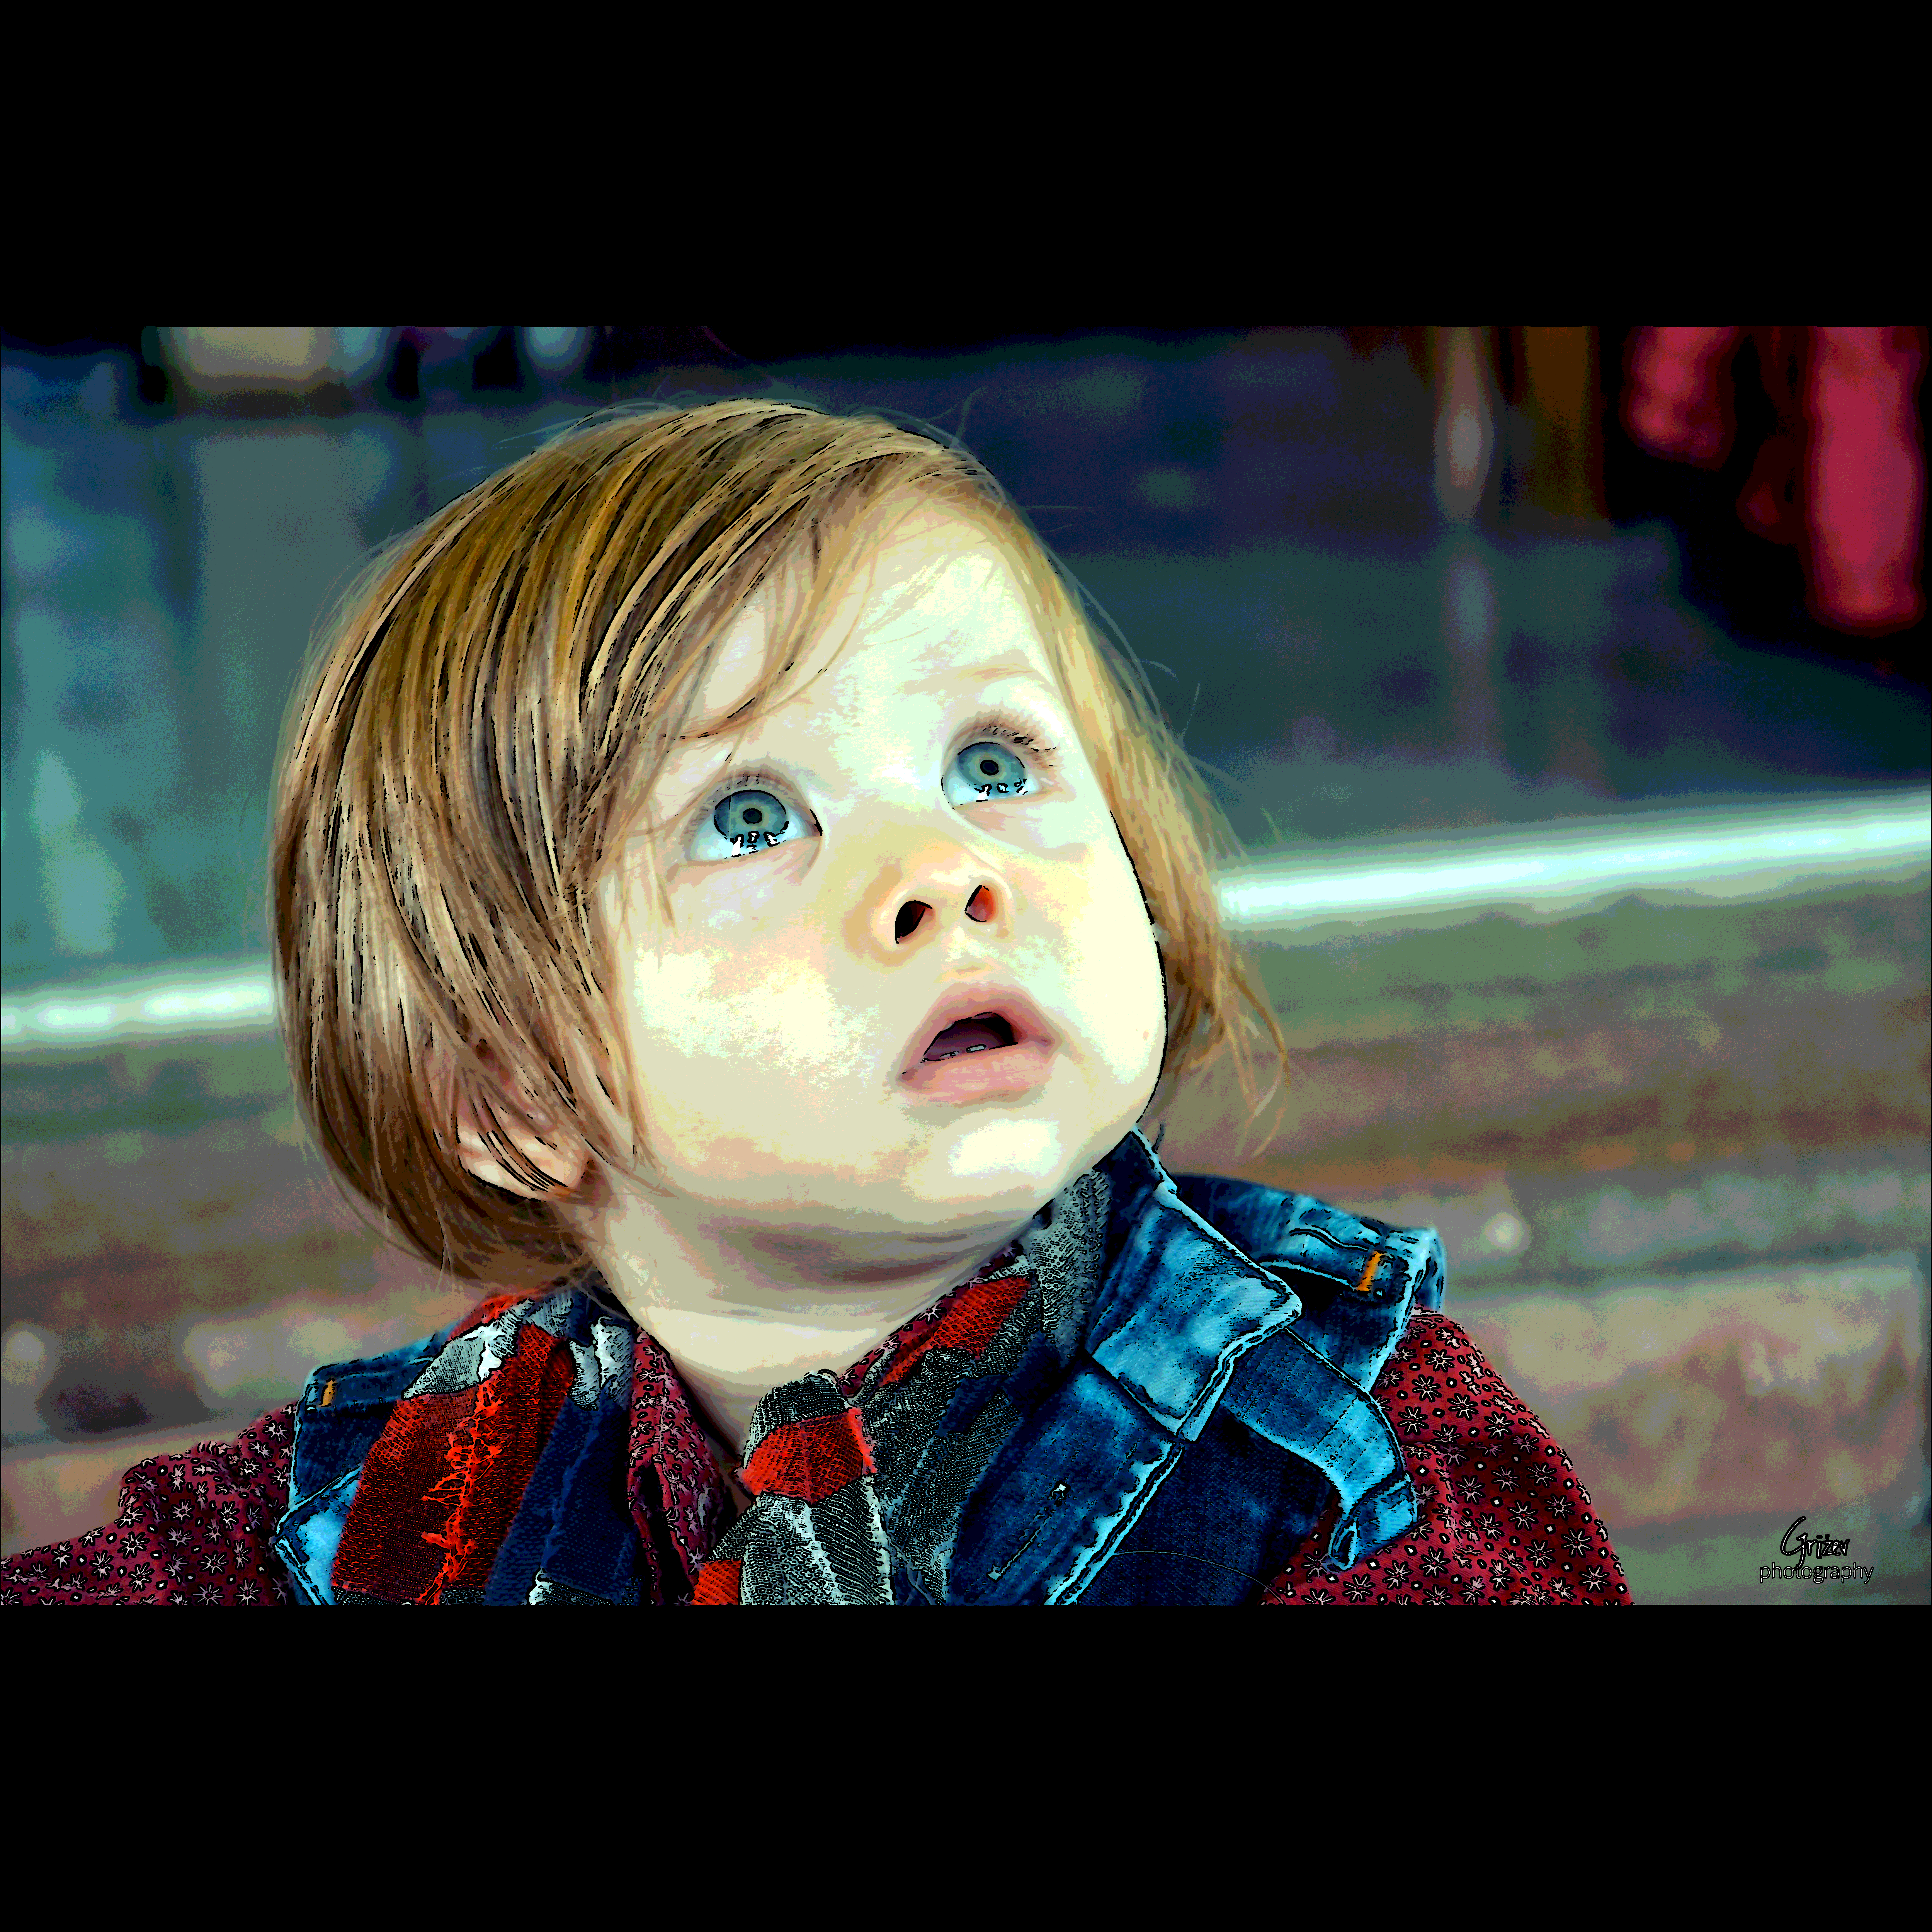
\includegraphics[width=\textwidth]{../resources/output_5000_5_9.jpg}
        \caption{Filtro $5 \times 5$, 9~niveles.}
        \label{fig:out_5000_5_9}
    \end{minipage}
    \caption{Resultados del procesamiento sobre la imagen de $5000 \times 5000$~píxeles.}
    \label{fig:output_5000}
\end{figure}

En la resolución máxima del benchmark, la tendencia se confirma de forma concluyente. La configuración liviana (Figura~\ref{fig:out_5000_3_3}) produce un resultado con una paleta de colores extremadamente reducida, donde los detalles finos se pierden por completo y las transiciones entre regiones de distinto color son bruscas y artificiales. La configuración pesada (Figura~\ref{fig:out_5000_5_9}) logra un equilibrio entre la estilización propia del posterizado y la preservación de la riqueza visual de la imagen original, demostrando que el aumento del número de niveles de cuantización es el factor determinante para obtener un resultado natural y visualmente agradable.
